\documentclass[pdftex,12pt,a4paper]{report}

\usepackage[portuguese,english]{babel}
\usepackage[T1]{fontenc} 
\usepackage[table,xcdraw]{xcolor}
\usepackage[utf8]{inputenc}
\usepackage[pdftex]{graphicx}
\usepackage{minitoc}
\usepackage{hyperref}
\usepackage{indentfirst}
\usepackage[compact]{titlesec}
\usepackage{fancyhdr}
\usepackage{caption}
\usepackage{pgfplots}
\usepackage{pgfplotstable}
\usepackage{fixltx2e}
\usepackage{mathtools}
\usepackage{fancyhdr}
\usepackage{listings}
\usepackage{color}
\usepackage{sverb}
\usepackage[section]{placeins}
\usepackage{adjustbox}
\titleformat*{\subsubsection}{\itshape}


%Highlight
\newcommand{\shellcmd}[1]{\indent\indent\texttt{\footnotesize\# #1}\\}

\pagestyle{fancy}
\renewcommand*\thesection{\thechapter\arabic{section}}
\newcommand{\HRule}{\rule{\linewidth}{0.5mm}}
\begin{document}

\begin{titlepage}

\begin{center}


\includegraphics[width=0.15\textwidth]{./logo}\\[0.5cm]    

\textsc{\large Universidade de Aveiro \\[1cm]\large departamento de electrónica, telecomunicações e informática}\\[1cm]

\textsc{\large{1}\large - Desempenho e Dimensionamento de Redes\\[1cm]}

\HRule \\[0.5cm]
{ \huge \bfseries abs}\\[0.4cm]
{ \large \bfseries x}\\[0.4cm]
\HRule \\[1cm]

\textsc{\small{8240 - MESTRADO INTEGRADO EM ENGENHARIA DE COMPUTADORES E TELEMÁTICA}}\\[1cm]

\begin{minipage}{0.4\textwidth}

\begin{flushleft} \large
\href{mailto:rafael.ferreira@ua.pt}{António Rafael da \\ Costa Ferreira }
 \small{\\NMec: 67405}
\end{flushleft}
\end{minipage}
\begin{minipage}{0.4\textwidth}

\begin{flushright} \large
\href{mailto:rodrigocunha@ua.pt}{Rodrigo Lopes \\ da Cunha}
\small{\\NMec: 67800}
\end{flushright}
\end{minipage}\\[1cm]

{\large Docente: Paulo Salvador }\\[0.5cm]

\vfill

{\large Fevereiro de 2016 \\ 2015-2016}

\end{center}

\end{titlepage} %Titulo do Relatorio
\renewcommand{\headrulewidth}{0pt}

%Cabeçalhos de rodapé
\fancyhead{}
\fancyfoot{}
\lhead{Network Traffic Engineering}
\rhead{DDR - 2015/2016}
\lfoot{Rafael Ferreira nmec: 67405 \\ Rodrigo Cunha nmec: 67800}
\rfoot{\thepage}

%Renomear Comandos
\renewcommand*\contentsname{Conteúdos}
\renewcommand*\figurename{Figura}
\renewcommand*\tablename{Tabela}

%Conteúdos, dar paragrafo
\tableofcontents
%Headers
\renewcommand{\headrulewidth}{0.15pt}
\renewcommand{\thechapter}{}



\clearpage

\section{Exercício 1}

Para iniciar este trabalho foi-nos dado vários ficheiros de base. O ficheiro NetGen.py é responsável por gerar uma rede, com vários nós que inclui o nome e localização geográfica, e as ligações inter-nó, matrizes de tráfego que define os fluxos de tráfego entre todas as cidades/ nós.

A localização geográfica (pos) é obtida dinamicamente a partir do nome do no (nome da cidade) usando a API do Google Maps, ficheiro getGeo.py. 

A matriz de tráfego (TM) é gerado aleatóriamente. É possível também guardar o resultado num ficheiro .dat e passando como argumento o parâmetro -f, net.dat.

\begin{figure}[!htb]
  \centering
  \begin{minipage}[b]{0.4\textwidth}
    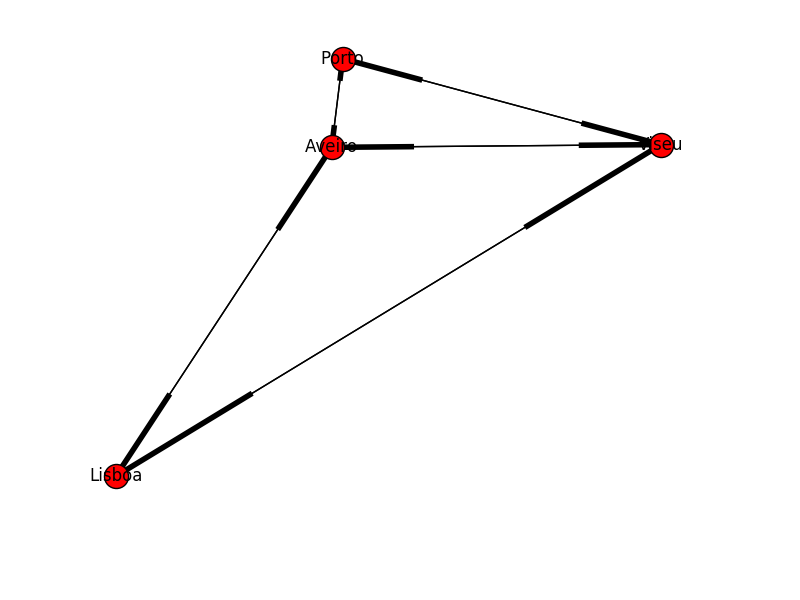
\includegraphics[width=\textwidth]{imagensGuia/esquema_rede_pequena.png}
  \end{minipage}
  \hfill
  \begin{minipage}[b]{0.4\textwidth}
    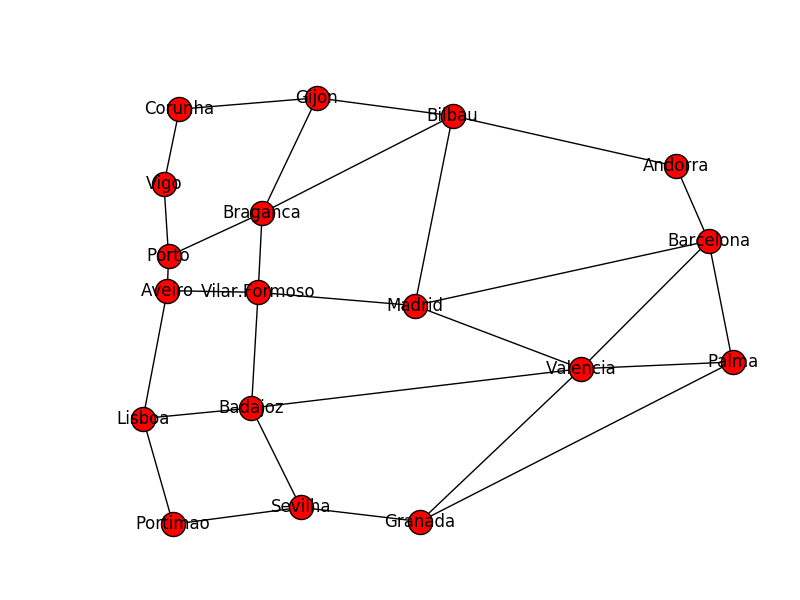
\includegraphics[width=\textwidth]{imagensGuia/esquema_rede_grande.png}
  \end{minipage}
  \caption{Rede pequena de teste e rede grande}
\end{figure}


\section{Exercício 2, 3 e 4}

No exercício 2 é usado o caminho mais curto como escolha para o caminho entre pontos, sendo que isto é dado pela soma das conexões e usando o algoritmo Greedy.

No exercício 3, foi calculado o "average one-way delay" e a carga em todas as direções em todos os links.

Para isso, para calcular o "average one-way delay", foi usada a seguinte fórmula baseada na aproximação Kleinrock:

$\mu$ = 1e9 / 8000 , é igual ao link speed em pkts/sec (1Gbps)

\[W = 1e6\times\left[\frac{1}{\left(\mu-atraso\right)}\right]\]

Para calcular o atraso, teve de se criar um ciclo de forma a percorrer todos os links e criar uma lista com os atrasos.

\begin{lstlisting}[language=python]
for pair in allpairs:
    path = sol[pair]
    for i in range(0, len(path) - 1):
        ws_delay[pair] = 1e6 / (mu - \
        net[path[i]][path[i + 1]]['load'])
\end{lstlisting}

Após isso foi possível apresentar a seguinte tabela para a rede pequena:

\begin{table}[!htb]
        \centering
        \resizebox{\textwidth}{!}{\begin{tabular}{|l|l|l|l|l|}
\hline
\multicolumn{1}{|c|}{\textbf{Origem}} & \multicolumn{1}{|c|}{\textbf{Destino}} & \multicolumn{1}{|c|}{\textbf{Saltos}} & \multicolumn{1}{|c|}{\textbf{Carga (pkts/sec)}} & \multicolumn{1}{|c|}{\textbf{Atraso (micro/sec)}} \\ \hline
Lisboa & Viseu & Lisboa, Viseu & 31271 & 10.67 \\ \hline
Porto & Lisboa & Porto, Aveiro, Lisboa & Indisponível & 31.86 \\ \hline
Viseu & Porto & Viseu, Porto & 31401 & 10.68 \\ \hline
Lisboa & Aveiro & Lisboa, Aveiro & 62675 & 16.04 \\ \hline
Aveiro & Viseu & Aveiro, Viseu & 31199 & 10.66 \\ \hline
Viseu & Aveiro & Viseu, Aveiro & 31378 & 10.68 \\ \hline
Aveiro & Porto & Aveiro, Porto & 63050 & 16.14 \\ \hline
Porto & Viseu & Porto, Viseu & 31396 & 10.68 \\ \hline
Porto & Aveiro & Porto, Aveiro & 62129 & 15.91 \\ \hline
Lisboa & Porto & Lisboa, Aveiro, Porto & Indisponível & 32.19 \\ \hline
Viseu & Lisboa & Viseu, Lisboa & 31171 & 10.66 \\ \hline
Aveiro & Lisboa & Aveiro, Lisboa & 62304 & 15.95 \\ \hline
\end{tabular}}
\caption[]{Solução obtida, carga nos links e atraso}
\end{table}



Analisando a tabela obtida conseguimos perceber que o link Aveiro-Porto tem o máximo delay de 16.14 micro segundos e a carga máxima está de Aveiro ao Porto com 63050 pacotes/ segundo.

\begin{table}[!htb]
        \centering
        \resizebox{\textwidth}{!}{\begin{tabular}{|l|l|l|}
\hline
\multicolumn{1}{|c|}{\textbf{Maximum one-way delay flow}} & \multicolumn{1}{|c|}{\textbf{Maximum one-way delay}} & \multicolumn{1}{|c|}{\textbf{Mean one-way delay}} \\ \hline
Aveiro-Porto & 16.1420500404 & 13.3475508848 \\ \hline
\end{tabular}}
\caption[]{Atraso}
\end{table}



\begin{table}[!htb]
        \centering
        \resizebox{\textwidth}{!}{\begin{tabular}{|l|l|l|}
\hline
\multicolumn{1}{|c|}{\textbf{Max load flow}} & \multicolumn{1}{|c|}{\textbf{Maximum one-way load}} & \multicolumn{1}{|c|}{\textbf{Mean one-way load}} \\ \hline
Aveiro-Porto & 63050.00 pkts/sec & 43797.40 pkts/sec \\ \hline
\end{tabular}}
\caption[]{Carga}
\end{table}



\newpage

\section{Exercício 5, 6 e 7}

No exercício 5 foi pedido que o routing agora fosse feito usando como parâmetro de escolha a menor carga possível, otimizando assim a largura de banda disponível  ao longo do caminho.

A nível de código, a única mudança efetuada importante foi:
\begin{lstlisting}[language=python]
path = nx.shortest_path(net, pair[0], pair[1], weight='load')
\end{lstlisting}

Pois agora o critério para escolha do caminho mais curto é a carga.

Para a rede pequena o resultado obtido foi:

\begin{table}[!htb]
        \centering
        \resizebox{\textwidth}{!}{\begin{tabular}{|l|l|l|l|l|}
\hline
\multicolumn{1}{|c|}{\textbf{Origem}} & \multicolumn{1}{|c|}{\textbf{Destino}} & \multicolumn{1}{|c|}{\textbf{Saltos}} & \multicolumn{1}{|c|}{\textbf{Carga (pkts/sec)}} & \multicolumn{1}{|c|}{\textbf{Atraso (micro/sec)}} \\ \hline
Lisboa & Viseu & Lisboa, Viseu & 62601 & 16.03 \\ \hline
Porto & Lisboa & Porto, Viseu, Lisboa & Indisponível & 15.95 \\ \hline
Viseu & Porto & Viseu, Porto & 62731 & 16.06 \\ \hline
Lisboa & Aveiro & Lisboa, Aveiro & 31345 & 10.68 \\ \hline
Aveiro & Viseu & Aveiro, Viseu & 31199 & 10.66 \\ \hline
Viseu & Aveiro & Viseu, Aveiro & 31378 & 10.68 \\ \hline
Aveiro & Porto & Aveiro, Porto & 31720 & 10.72 \\ \hline
Porto & Viseu & Porto, Viseu & 62512 & 16.00 \\ \hline
Porto & Aveiro & Porto, Aveiro & 31013 & 10.64 \\ \hline
Lisboa & Porto & Lisboa, Viseu, Porto & Indisponível & 16.06 \\ \hline
Viseu & Lisboa & Viseu, Lisboa & 62287 & 15.95 \\ \hline
Aveiro & Lisboa & Aveiro, Lisboa & 31188 & 10.66 \\ \hline
\end{tabular}}
\caption[]{Solução obtida, carga nos links e atraso}
\end{table}



Analisando a tabela e os resultados obtidos conseguimos perceber que houve mudança na distribuição dos caminhos mais curtos, por exemplo, Porto > Lisboa agora o caminho é feito por Porto, Viseu e Lisboa, já de Lisboa > Porto é feito por Lisboa, Viseu, Porto.

Este resultado é explicado porque a lista de pares da rede pequena está distribuída da seguinte forma:

\begin{lstlisting}[language=python]
[('Lisboa', 'Viseu'), ('Lisboa', 'Aveiro'),
('Lisboa', 'Porto'), ('Viseu', 'Lisboa'), ('Viseu', 'Aveiro'),
('Viseu', 'Porto'), ('Aveiro', 'Lisboa'), ('Aveiro', 'Viseu'), 
('Aveiro', 'Porto'), ('Porto', 'Lisboa'), ('Porto', 'Viseu'),
('Porto', 'Aveiro')]
\end{lstlisting}

Inicialmente, irá testar a ligação Lisboa > Viseu, à qual será atribuída, depois Lisboa > Aveiro e será também atribuída, de seguida, Lisboa > Porto, como o somatório das cargas entre as ligações Lisboa > Viseu (31271) + Viseu > Porto (0) tem menos carga do que a Lisboa > Aveiro (31345) + Aveiro > Porto (0) então seleciona ir por Viseu, daí a diferença nos resultados em relação ao primeiro exercício.
 
Na diferença de Porto > Lisboa, temos Porto > Aveiro (0)  + Aveiro > Lisboa (31188) com mais carga do que Porto > Viseu (0) + Viseu > Lisboa (31171) no momento de atribuição, o que faz com que seja selecionado o caminho: Porto > Viseu > Lisboa.

\begin{table}[!htb]
        \centering
        \resizebox{\textwidth}{!}{\begin{tabular}{|l|l|l|}
\hline
\multicolumn{1}{|c|}{\textbf{Maximum one-way delay flow}} & \multicolumn{1}{|c|}{\textbf{Maximum one-way delay}} & \multicolumn{1}{|c|}{\textbf{Mean one-way delay}} \\ \hline
Lisboa-Porto & 32.0852532284 & 16.0089473288 \\ \hline
\end{tabular}}
\caption[]{Atraso}
\end{table}



\begin{table}[!htb]
        \centering
        \resizebox{\textwidth}{!}{\begin{tabular}{|l|l|l|}
\hline
\multicolumn{1}{|c|}{\textbf{Max load flow}} & \multicolumn{1}{|c|}{\textbf{Maximum one-way load}} & \multicolumn{1}{|c|}{\textbf{Mean one-way load}} \\ \hline
Viseu-Porto & 62731.00 pkts/sec & 43797.40 pkts/sec \\ \hline
\end{tabular}}
\caption[]{Carga}
\end{table}



Com este exercício, mudando o critério para carga nos links na escolha do caminho mais curto, conseguimos melhorias no "maximum one-way delay" (-0,083 microseg) de  e no "maximum one-way load" (-319 pkts\/sec). 

%16.1420500404-16.0593553775=0,0826946629 micro sec
%63050.00-62731.00=319 pkts/sec

\section{Exercício 8, 9 e 10}

No exercício 8 pretende-se que seja escolhido o caminho mais curto tendo em conta o atraso, minimizando assim o "average one-way delay". Este por sua vez irá sempre escolher de forma sequencial, o que fará com que seja sempre na mesma ordem.

A nível de código, a única mudança efetuada importante foi:
\begin{lstlisting}[language=python]
path = nx.shortest_path(net, pair[0], pair[1],
	 weight='delay')
...
net[path[i]][path[i + 1]]['delay'] = 1e6 / 
	(mu - net[path[i]][path[i + 1]]['load'])
\end{lstlisting}

\newpage

O critério agora é o atraso, e para calcular o atraso usou-se a aproximação M/M/1.

Para a rede pequena o resultado obtido foi:

\begin{table}[!htb]
        \centering
        \resizebox{\textwidth}{!}{\begin{tabular}{|l|l|l|l|l|}
\hline
\multicolumn{1}{|c|}{\textbf{Origem}} & \multicolumn{1}{|c|}{\textbf{Destino}} & \multicolumn{1}{|c|}{\textbf{Saltos}} & \multicolumn{1}{|c|}{\textbf{Carga (pkts/sec)}} & \multicolumn{1}{|c|}{\textbf{Atraso (micro/sec)}} \\ \hline
Lisboa & Viseu & Lisboa, Viseu & 62601 & 16.03 \\ \hline
Porto & Lisboa & Porto, Viseu, Lisboa & Indisponível & 15.95 \\ \hline
Viseu & Porto & Viseu, Porto & 62731 & 16.06 \\ \hline
Lisboa & Aveiro & Lisboa, Aveiro & 31345 & 10.68 \\ \hline
Aveiro & Viseu & Aveiro, Viseu & 31199 & 10.66 \\ \hline
Viseu & Aveiro & Viseu, Aveiro & 31378 & 10.68 \\ \hline
Aveiro & Porto & Aveiro, Porto & 31720 & 10.72 \\ \hline
Porto & Viseu & Porto, Viseu & 62512 & 16.00 \\ \hline
Porto & Aveiro & Porto, Aveiro & 31013 & 10.64 \\ \hline
Lisboa & Porto & Lisboa, Viseu, Porto & Indisponível & 16.06 \\ \hline
Viseu & Lisboa & Viseu, Lisboa & 62287 & 15.95 \\ \hline
Aveiro & Lisboa & Aveiro, Lisboa & 31188 & 10.66 \\ \hline
\end{tabular}}
\caption[]{Solução obtida, carga nos links e atraso}
\end{table}



Nesta tabela em relação ao exercício anterior não houve mudanças, isto devido à ordem ser a mesma de atribuição.

\begin{table}[!htb]
        \centering
        \resizebox{\textwidth}{!}{\begin{tabular}{|l|l|l|}
\hline
\multicolumn{1}{|c|}{\textbf{Maximum one-way delay flow}} & \multicolumn{1}{|c|}{\textbf{Maximum one-way delay}} & \multicolumn{1}{|c|}{\textbf{Mean one-way delay}} \\ \hline
Lisboa-Porto & 32.0852532284 & 16.0089473288 \\ \hline
\end{tabular}}
\caption[]{Atraso}
\end{table}



\begin{table}[!htb]
        \centering
        \resizebox{\textwidth}{!}{\begin{tabular}{|l|l|l|}
\hline
\multicolumn{1}{|c|}{\textbf{Max load flow}} & \multicolumn{1}{|c|}{\textbf{Maximum one-way load}} & \multicolumn{1}{|c|}{\textbf{Mean one-way load}} \\ \hline
Viseu-Porto & 16.06 pkts/sec & 12.81 pkts/sec \\ \hline
\end{tabular}}
\caption[]{Carga}
\end{table}



Como se pode observar, para a rede pequena manteve-se igual.

\begin{table}[!htb]
        \centering
        \resizebox{\textwidth}{!}{\begin{tabular}{|l|l|l|}
\hline
\multicolumn{1}{|c|}{\textbf{Maximum one-way delay flow}} & \multicolumn{1}{|c|}{\textbf{Maximum one-way delay}} & \multicolumn{1}{|c|}{\textbf{Mean one-way delay}} \\ \hline
Valencia-Badajoz & 79.2209331482 & 27.922949817 \\ \hline
\end{tabular}}
\caption[]{Atraso}
\end{table}



\begin{table}[!htb]
        \centering
        \resizebox{\textwidth}{!}{\begin{tabular}{|l|l|l|}
\hline
\multicolumn{1}{|c|}{\textbf{Max load flow}} & \multicolumn{1}{|c|}{\textbf{Maximum one-way load}} & \multicolumn{1}{|c|}{\textbf{Mean one-way load}} \\ \hline
Aveiro-Porto & 11.16 pkts/sec & 9.82 pkts/sec \\ \hline
\end{tabular}}
\caption[]{Carga}
\end{table}





\newpage

\end{document}



